%Suggested order of slides:

%1 slides-basics-whatisml
%2 slides-basics-data
%3 slides-basics-task
%4 slides-basics-models-parameters
%5 slides-basics-learner
%6 slides-basics-riskminimization
%7 slides-basics-optimization
%8 slides-basics-learnercomponents-hro

%slides-basics-notation is just a glossary, superseded by cheatsheet.

\subsection{What is Machine Learning?}
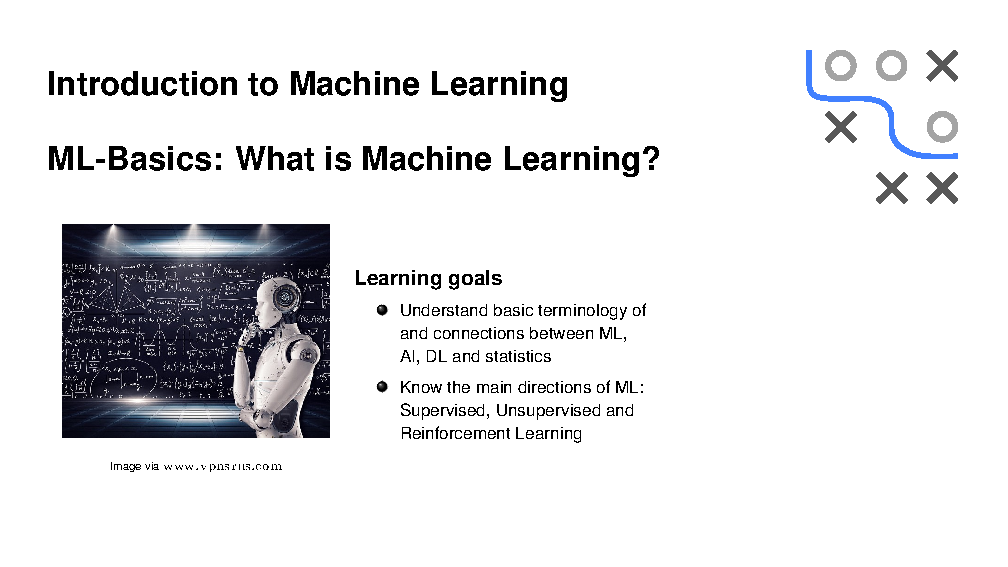
\includepdf[pages=-]{../slides-pdf/slides-basics-whatisml.pdf}

\subsection{Data}
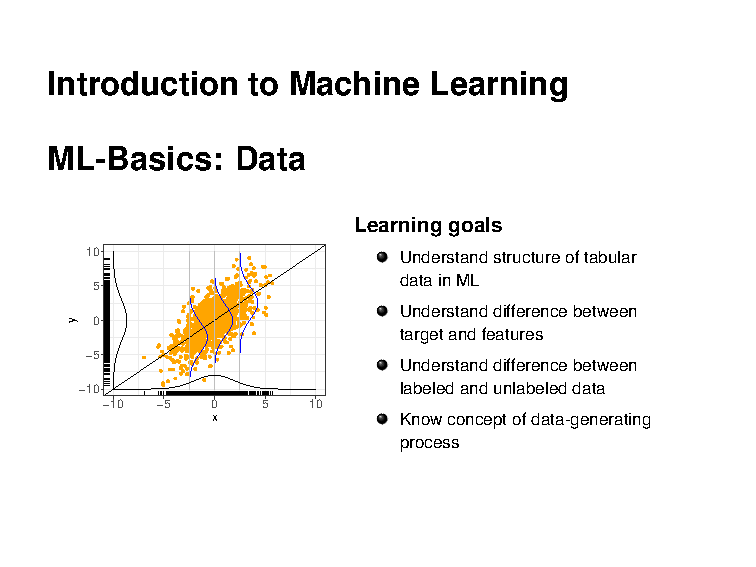
\includepdf[pages=-]{../slides-pdf/slides-basics-data.pdf}

\subsection{Supervised Tasks}
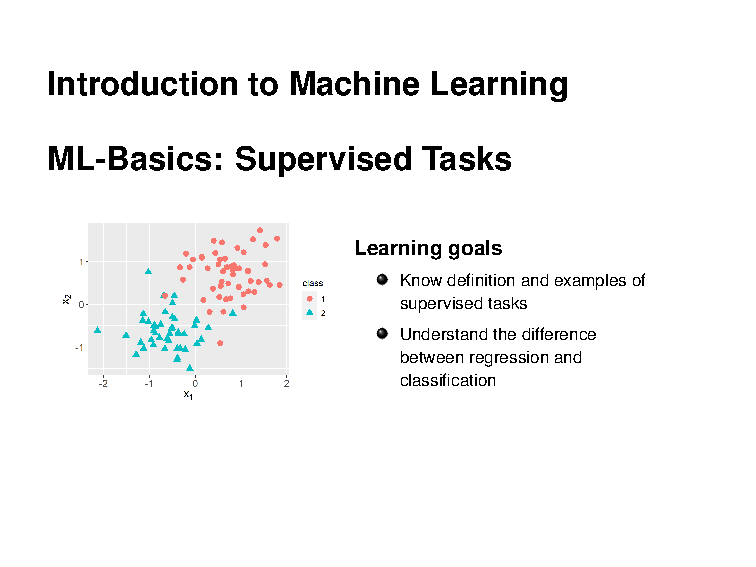
\includepdf[pages=-]{../slides-pdf/slides-basics-task.pdf}

\subsection{Models and Parameters}
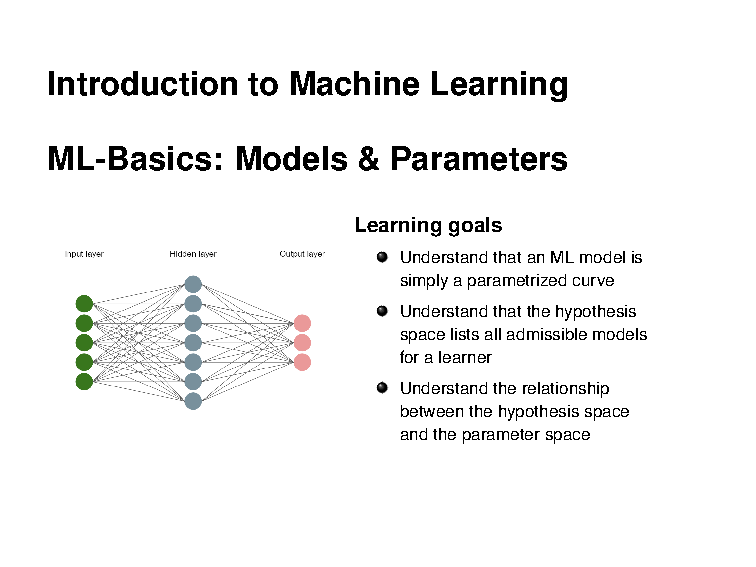
\includepdf[pages=-]{../slides-pdf/slides-basics-models-parameters.pdf}

\subsection{Learner}
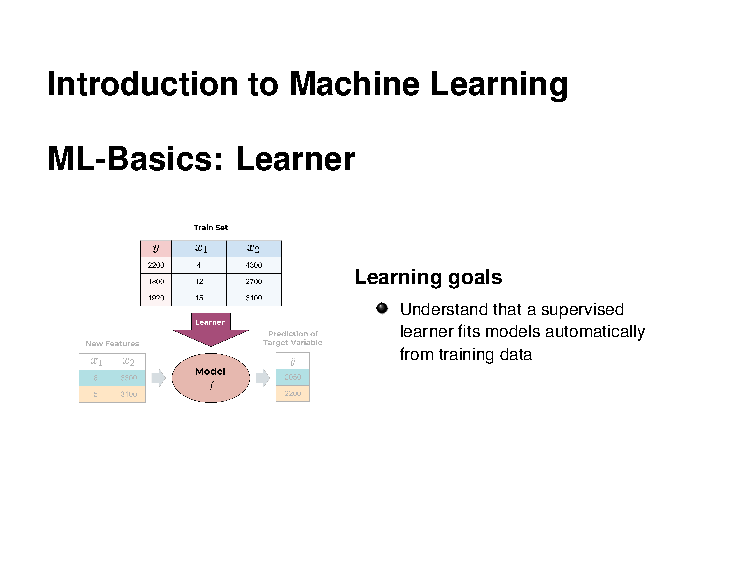
\includepdf[pages=-]{../slides-pdf/slides-basics-learner.pdf}

\subsection{Losses and Risk Minimization}
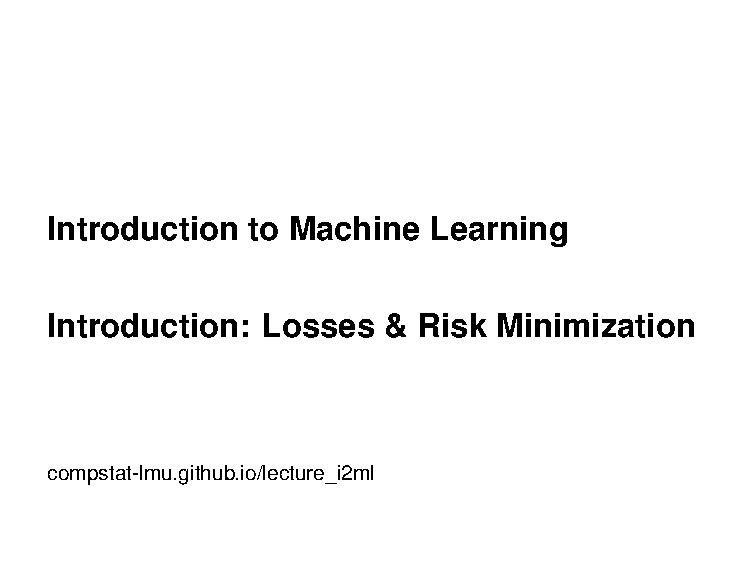
\includepdf[pages=-]{../slides-pdf/slides-basics-riskminimization.pdf}

\subsection{Optimization}
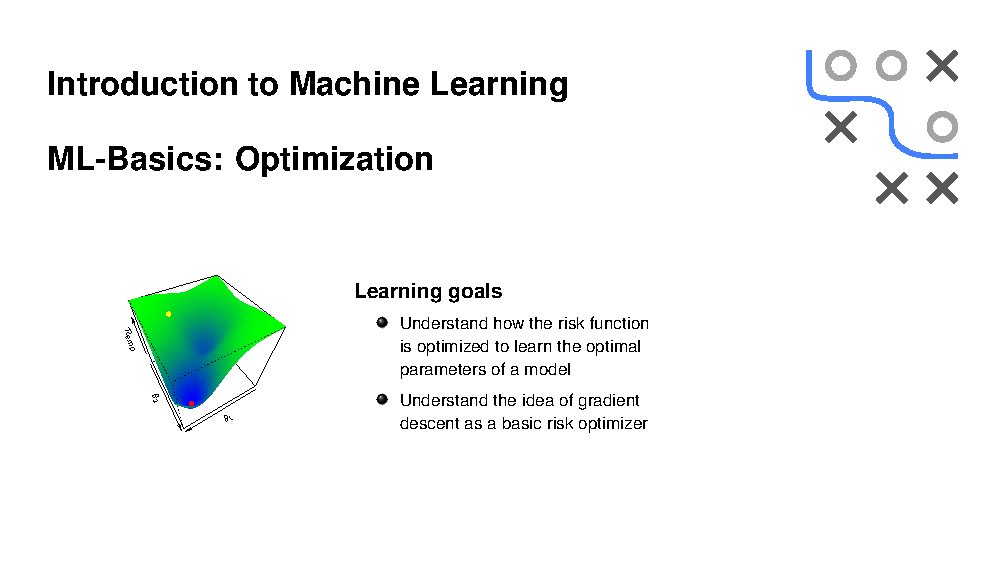
\includepdf[pages=-]{../slides-pdf/slides-basics-optimization.pdf}

\subsection{Components of Supervised Learning}
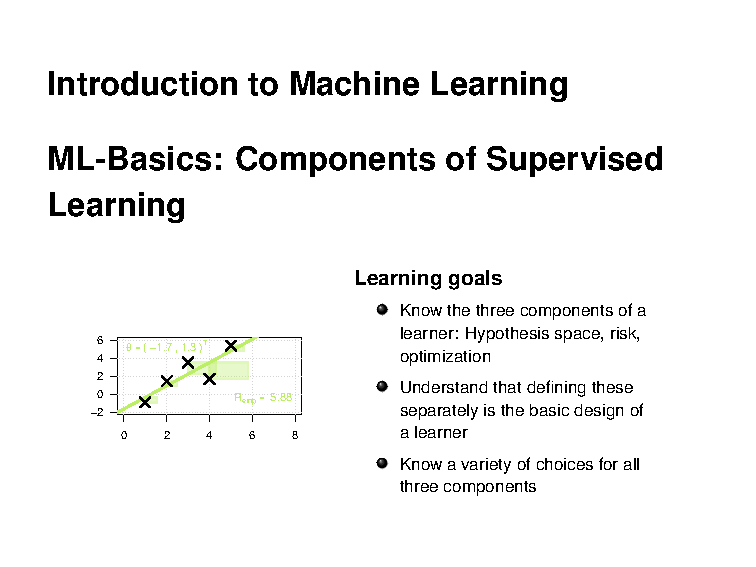
\includepdf[pages=-]{../slides-pdf/slides-basics-learnercomponents-hro.pdf}

